% ============================================================================
%  Figure 1 — Teaser (Step 6 of paper-writing workflow)
%  ----------------------------------------------------------------------------
%  Two-panel headline figure. Left: mean MC ASR vs cone dim k.
%  Right: mean KL retention vs k, with surgicality threshold 0.1.
%  Same color per model across both panels.
%
%  Required packages:
%     \usepackage{pgfplots}
%     \pgfplotsset{compat=1.18}
%     \usepackage{xcolor}
%
%  Data is hard-coded from results_summary.json (Exp 3 and Exp 5).
% ============================================================================

\begin{figure}[t]
\centering
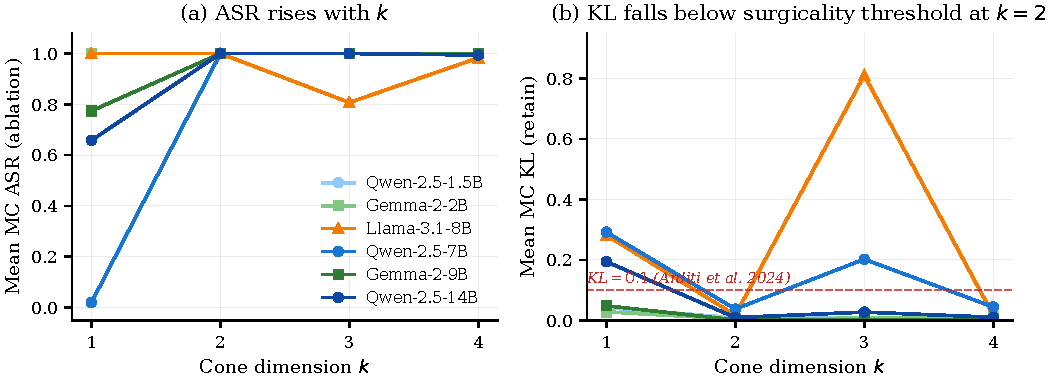
\includegraphics[width=\linewidth]{figures/fig_teaser.pdf}
% \definecolor{qw15}{HTML}{90CAF9}   % qwen-2.5-1.5b   light blue
% \definecolor{qw7}{HTML}{1976D2}    % qwen-2.5-7b     mid blue
% \definecolor{qw14}{HTML}{0D47A1}   % qwen-2.5-14b    deep blue
% \definecolor{gm2}{HTML}{81C784}    % gemma-2-2b      light green
% \definecolor{gm9}{HTML}{2E7D32}    % gemma-2-9b      deep green
% \definecolor{ll8}{HTML}{F57C00}    % llama-3.1-8b    orange
% \definecolor{thresholdred}{HTML}{C62828}

% \begin{tikzpicture}

% % --- LEFT PANEL: mean MC ASR (in-distribution, ablation) vs k ---------------
% \begin{axis}[
%     name=asrplot,
%     width=0.50\linewidth, height=5.5cm,
%     xlabel={Cone dimension $k$},
%     ylabel={Mean MC ASR (ablation)},
%     xmin=0.8, xmax=4.2,
%     ymin=-0.05, ymax=1.10,
%     xtick={1,2,3,4},
%     ytick={0, 0.25, 0.5, 0.75, 1.0},
%     grid=both, grid style={gray!20, line width=0.3pt},
%     legend style={font=\scriptsize, at={(0.55,0.36)}, anchor=north,
%                   draw=gray!50, fill=white, fill opacity=0.85,
%                   text opacity=1, row sep=-2pt},
%     legend cell align=left,
%     tick label style={font=\scriptsize},
%     label style={font=\small},
%     title={\small \textbf{(a)} ASR rises with $k$},
%     title style={yshift=-1ex},
%     every axis plot/.append style={line width=0.9pt, mark size=2pt}
% ]

% % qwen-2.5-1.5b
% \addplot[color=qw15, mark=*]        coordinates {(1,1.000)(2,1.000)(3,1.000)(4,1.000)};
% % gemma-2-2b
% \addplot[color=gm2, mark=square*]   coordinates {(1,1.000)(2,1.000)(3,1.000)(4,1.000)};
% % llama-3.1-8b
% \addplot[color=ll8, mark=triangle*] coordinates {(1,1.000)(2,1.000)(3,0.807)(4,0.983)};
% % qwen-2.5-7b
% \addplot[color=qw7, mark=*]         coordinates {(1,0.020)(2,1.000)(3,1.000)(4,1.000)};
% % gemma-2-9b
% \addplot[color=gm9, mark=square*]   coordinates {(1,0.774)(2,1.000)(3,1.000)(4,1.000)};
% % qwen-2.5-14b
% \addplot[color=qw14, mark=*]        coordinates {(1,0.658)(2,1.000)(3,1.000)(4,0.994)};

% \legend{Qwen-2.5-1.5B, Gemma-2-2B, Llama-3.1-8B,
%         Qwen-2.5-7B, Gemma-2-9B, Qwen-2.5-14B}
% \end{axis}


% % --- RIGHT PANEL: mean MC KL on retain set vs k -----------------------------
% \begin{axis}[
%     at={($(asrplot.east) + (1.4cm,0)$)}, anchor=west,
%     width=0.50\linewidth, height=5.5cm,
%     xlabel={Cone dimension $k$},
%     ylabel={Mean MC KL (retain)},
%     xmin=0.8, xmax=4.2,
%     ymin=0, ymax=0.95,
%     xtick={1,2,3,4},
%     ytick={0, 0.1, 0.25, 0.5, 0.75},
%     extra y ticks={0.1},
%     extra y tick labels={},
%     extra y tick style={grid=major, grid style={thresholdred, dashed, line width=0.8pt}},
%     grid=both, grid style={gray!20, line width=0.3pt},
%     tick label style={font=\scriptsize},
%     label style={font=\small},
%     title={\small \textbf{(b)} KL falls below surgicality threshold at $k{=}2$},
%     title style={yshift=-1ex},
%     every axis plot/.append style={line width=0.9pt, mark size=2pt}
% ]

% % Threshold callout
% \node[font=\scriptsize\itshape, text=thresholdred, anchor=west]
%     at (axis cs:0.85, 0.135) {KL $= 0.1$ (Arditi et al.~2024)};

% % qwen-2.5-1.5b
% \addplot[color=qw15, mark=*]        coordinates {(1,0.042)(2,0.008)(3,0.009)(4,0.008)};
% % gemma-2-2b
% \addplot[color=gm2,  mark=square*]  coordinates {(1,0.028)(2,0.004)(3,0.007)(4,0.012)};
% % llama-3.1-8b
% \addplot[color=ll8,  mark=triangle*] coordinates {(1,0.282)(2,0.017)(3,0.811)(4,0.017)};
% % qwen-2.5-7b
% \addplot[color=qw7,  mark=*]        coordinates {(1,0.292)(2,0.037)(3,0.202)(4,0.044)};
% % gemma-2-9b
% \addplot[color=gm9,  mark=square*]  coordinates {(1,0.048)(2,0.001)(3,0.001)(4,0.002)};
% % qwen-2.5-14b
% \addplot[color=qw14, mark=*]        coordinates {(1,0.194)(2,0.009)(3,0.027)(4,0.010)};

% \end{axis}
% \end{tikzpicture}

\caption{%
\textbf{$k=2$ resolves both axes simultaneously for larger models.}
\textbf{(a)} Mean Monte-Carlo Answer Switching Rate over $32$ directions sampled
from the learned cone (in-distribution ablation) versus cone dimension $k$.
For smaller models (Qwen-2.5-1.5B, Gemma-2-2B, Llama-3.1-8B) a $1$-dim direction
already saturates; for Qwen-2.5-7B/14B and Gemma-2-9B a $1$-dim direction is
causally insufficient, but $k{=}2$ closes the gap.
\textbf{(b)} Mean KL divergence on $100$ retain prompts (last $30$ token
positions). The same three larger models that suffered low ASR at $k{=}1$ also
\emph{exceed} the surgicality threshold $\mathrm{KL}=0.1$ (red dashed line) at
$k{=}1$, and \emph{all} fall below it at $k{=}2$. Across these models, the
$k{=}2$ cone is both more effective and less destructive than the $1$-D probe.
Llama-3.1-8B and
Qwen-2.5-7B regress at $k{=}3$, identifying $k{=}2$ as the safe operating point.
}
\label{fig:teaser}
\end{figure}
